% (C) Marc Lijour, 2016-2017
% Licensed under a Creative Commons License BY-SA
% https://creativecommons.org/licenses/by-sa/2.5/ca/
% Presentation for the Small Business Digitization Initiative (SBDI) training program
% see http://www.ictc-ctic.ca/small-business-digitization-initiative/ 
% authored by Marc Lijour, December 2016
% for the session running from January 2017 to September 2017
% 
% Variables
% TODO set the variables
% ---------------------- USER-DEFINED --------------------------------
\newcommand{\SFLtitle}{Digitization~Theory~3}
\newcommand{\SFLlongtitle}{Creating Value with Software}
\newcommand{\SFLsubtitle}{Small Business Digitization Initiative (SBDI) - Day 3}
\newcommand{\SFLauthor}{Marc~Lijour}
\newcommand{\SFLdate}{March~22, 2017}
\newcommand{\SFLsubject}{Digitization Theory}
% --------------------------------------------------------------------
% Template
% (C) Savoir-faire Linux, 2016 (this document and associated logos and art)
% This document is licensed under a Creative Commons License BY-SA (feel free to use the code, but all rights are reserved for logos and art)
% https://creativecommons.org/licenses/by-sa/2.5/ca/
% Savoir-faire Linux presentation template for LaTeX
% authored by Marc Lijour, December 2016
% This template comes with a first page on a blue background
% Possible improvement in future iterations
% - Test and fix as needed to work on xetex (to use Ubuntu fonts)
% === USAGE===
% Create a file for your LaTeX content (slides, etc), in which you must do the following:
% TODO 1 - set variables defined below
% TODO 2 - include this code by calling: % (C) Savoir-faire Linux, 2016 (this document and associated logos and art)
% This document is licensed under a Creative Commons License BY-SA (feel free to use the code, but all rights are reserved for logos and art)
% https://creativecommons.org/licenses/by-sa/2.5/ca/
% Savoir-faire Linux presentation template for LaTeX
% authored by Marc Lijour, December 2016
% This template comes with a first page on a blue background
% Possible improvement in future iterations
% - Test and fix as needed to work on xetex (to use Ubuntu fonts)
% === USAGE===
% Create a file for your LaTeX content (slides, etc), in which you must do the following:
% TODO 1 - set variables defined below
% TODO 2 - include this code by calling: % (C) Savoir-faire Linux, 2016 (this document and associated logos and art)
% This document is licensed under a Creative Commons License BY-SA (feel free to use the code, but all rights are reserved for logos and art)
% https://creativecommons.org/licenses/by-sa/2.5/ca/
% Savoir-faire Linux presentation template for LaTeX
% authored by Marc Lijour, December 2016
% This template comes with a first page on a blue background
% Possible improvement in future iterations
% - Test and fix as needed to work on xetex (to use Ubuntu fonts)
% === USAGE===
% Create a file for your LaTeX content (slides, etc), in which you must do the following:
% TODO 1 - set variables defined below
% TODO 2 - include this code by calling: \input{sfl-presentation-template-blue-EN}
% TODO 3 - Start the document as usual and you're in business; just use \begin{document} and don't forget to conclude with \end{document}
% TODO 4 - Use the custom method \SFLcoverpage instead of \titlepage to create your cover page
% Voilà!
%
\documentclass{beamer}
\usepackage{etoolbox}
% Variables
% ---------------------- USER-DEFINED --------------------------------
\ifdef{\SFLtitle}{}{\newcommand{\SFLtitle}{\color{red}Title TBD}}
\ifdef{\SFLlongtitle}{}{\newcommand{\SFLlongtitle}{\color{red}Long title TBD}}
\ifdef{\SFLsubtitle}{}{\newcommand{\SFLsubtitle}{\color{red}Subtitle TBD}}
\ifdef{\SFLauthor}{}{\newcommand{\SFLauthor}{\color{red}Author TBD}}
\ifdef{\SFLdate}{}{\newcommand{\SFLdate}{\color{red}Date TBD}}
\ifdef{\SFLsubject}{}{\newcommand{\SFLsubject}{\color{red}Subject TBD}}
% --------------------------------------------------------------------
\usetheme{Boadilla}
% Set color close to Savoir-faire Linux standard
\definecolor{beamer@blendedblue}{RGB}{86,176,201}
% Cover Page
\title[\SFLtitle] {\SFLlongtitle}
\subtitle{\SFLsubtitle}
\author{\SFLauthor}
\date{\SFLdate}
\subject{\SFLsubject}
\usepackage{tikz}
% -- possible approach through modif of the template (abandonned for now)
%\addtobeamertemplate{title page}{
%    \tikz[remember picture,overlay]
%        \node at ([xshift=0cm,yshift=0cm]current page.center) 
%		 {
\includegraphics[width=\paperwidth, height=\paperheight]{./images/sfl-background-blue}};
%}{}
%\setbeamercolor{title page}{fg=white}
%\setbeamercolor{titlelike}{fg=white}
%\setbeamertemplate{navigation symbols}{}
% Try Xetex to use system fonts (pdflatex makes it hard to import a font)
%\usepackage{fontspec}
%\setsansfont{Ubuntu}
%\setmonofont{Ubuntu Mono}
%
%\usepackage[absolute,overlay]{textpos}
%\setlength{\TPHorizModule}{\paperwidth}
%\setlength{\TPVertModule}{\paperheight}
% -- create a custom (command) title page -which has the benefit of not affecting the settings for the rest of the presentation
\newcommand{\SFLcoverpage}{\frame[plain]{
	\tikz[remember picture,overlay] {
        	\node(bkgd) at ([xshift=0cm,yshift=0cm]current page.center) 
			{
\includegraphics[width=\paperwidth, height=\paperheight]{../templates/images/sfl-background-blue}};
        	\node(logo) at ([xshift=0cm,yshift=2.5cm]current page.center) 
		 	{
\includegraphics[scale=.20]{../templates/images/logo-sfl-blanc-rgb-72dpi}};
	}
	\tikz[remember picture,overlay] {
        	\node(title) at ([xshift=0cm,yshift=1cm]current page.center) 
			{\Large\color{white}\textbf{{\SFLlongtitle}}};
        	\node(subtitle) at ([xshift=0cm,yshift=.2cm]current page.center) 
			{\small\color{white}\emph{\SFLsubtitle}};
        	\node(author) at ([xshift=0cm,yshift=-2cm]current page.center) 
			{\small\color{white}By~\SFLauthor};
        	\node(date) at ([xshift=0cm,yshift=-2.5cm]current page.center) 
			{\tiny\color{white}\SFLdate};
        	\node(footnote) at ([xshift=0cm,yshift=-4cm]current page.center) 
			{\TINY\color{white}\emph{The registered trademark Linux$^\circledR$ is used pursuant to a sublicense from LMI, the exclusive licensee of Linus Torvalds, owner of the mark on a world-wide basis.}};
    	}
}}
%
% This sets a Savoir-faire Linux logo at the bottom right corner of each page
\logo{
\includegraphics[scale=.1]{../templates/images/logo-sfl-250.png}}
\AtBeginSection[]
{
  \begin{frame}
    \frametitle{Table of Contents}
    \tableofcontents[currentsection]
  \end{frame}
}
%\usepackage[format=plain,justification=raggedright,singlelinecheck=false]{caption}
\usepackage[format=plain,justification=justified,singlelinecheck=false]{caption}
\usepackage[utf8]{inputenc}
\usepackage{dirtytalk}
\usepackage{wrapfig}
\usepackage{hyperref}
\usepackage{verbatim}
\usepackage{mathabx}
%\usepackage{MnSymbol}


% TODO 3 - Start the document as usual and you're in business; just use \begin{document} and don't forget to conclude with \end{document}
% TODO 4 - Use the custom method \SFLcoverpage instead of \titlepage to create your cover page
% Voilà!
%
\documentclass{beamer}
\usepackage{etoolbox}
% Variables
% ---------------------- USER-DEFINED --------------------------------
\ifdef{\SFLtitle}{}{\newcommand{\SFLtitle}{\color{red}Title TBD}}
\ifdef{\SFLlongtitle}{}{\newcommand{\SFLlongtitle}{\color{red}Long title TBD}}
\ifdef{\SFLsubtitle}{}{\newcommand{\SFLsubtitle}{\color{red}Subtitle TBD}}
\ifdef{\SFLauthor}{}{\newcommand{\SFLauthor}{\color{red}Author TBD}}
\ifdef{\SFLdate}{}{\newcommand{\SFLdate}{\color{red}Date TBD}}
\ifdef{\SFLsubject}{}{\newcommand{\SFLsubject}{\color{red}Subject TBD}}
% --------------------------------------------------------------------
\usetheme{Boadilla}
% Set color close to Savoir-faire Linux standard
\definecolor{beamer@blendedblue}{RGB}{86,176,201}
% Cover Page
\title[\SFLtitle] {\SFLlongtitle}
\subtitle{\SFLsubtitle}
\author{\SFLauthor}
\date{\SFLdate}
\subject{\SFLsubject}
\usepackage{tikz}
% -- possible approach through modif of the template (abandonned for now)
%\addtobeamertemplate{title page}{
%    \tikz[remember picture,overlay]
%        \node at ([xshift=0cm,yshift=0cm]current page.center) 
%		 {
\includegraphics[width=\paperwidth, height=\paperheight]{./images/sfl-background-blue}};
%}{}
%\setbeamercolor{title page}{fg=white}
%\setbeamercolor{titlelike}{fg=white}
%\setbeamertemplate{navigation symbols}{}
% Try Xetex to use system fonts (pdflatex makes it hard to import a font)
%\usepackage{fontspec}
%\setsansfont{Ubuntu}
%\setmonofont{Ubuntu Mono}
%
%\usepackage[absolute,overlay]{textpos}
%\setlength{\TPHorizModule}{\paperwidth}
%\setlength{\TPVertModule}{\paperheight}
% -- create a custom (command) title page -which has the benefit of not affecting the settings for the rest of the presentation
\newcommand{\SFLcoverpage}{\frame[plain]{
	\tikz[remember picture,overlay] {
        	\node(bkgd) at ([xshift=0cm,yshift=0cm]current page.center) 
			{
\includegraphics[width=\paperwidth, height=\paperheight]{../templates/images/sfl-background-blue}};
        	\node(logo) at ([xshift=0cm,yshift=2.5cm]current page.center) 
		 	{
\includegraphics[scale=.20]{../templates/images/logo-sfl-blanc-rgb-72dpi}};
	}
	\tikz[remember picture,overlay] {
        	\node(title) at ([xshift=0cm,yshift=1cm]current page.center) 
			{\Large\color{white}\textbf{{\SFLlongtitle}}};
        	\node(subtitle) at ([xshift=0cm,yshift=.2cm]current page.center) 
			{\small\color{white}\emph{\SFLsubtitle}};
        	\node(author) at ([xshift=0cm,yshift=-2cm]current page.center) 
			{\small\color{white}By~\SFLauthor};
        	\node(date) at ([xshift=0cm,yshift=-2.5cm]current page.center) 
			{\tiny\color{white}\SFLdate};
        	\node(footnote) at ([xshift=0cm,yshift=-4cm]current page.center) 
			{\TINY\color{white}\emph{The registered trademark Linux$^\circledR$ is used pursuant to a sublicense from LMI, the exclusive licensee of Linus Torvalds, owner of the mark on a world-wide basis.}};
    	}
}}
%
% This sets a Savoir-faire Linux logo at the bottom right corner of each page
\logo{
\includegraphics[scale=.1]{../templates/images/logo-sfl-250.png}}
\AtBeginSection[]
{
  \begin{frame}
    \frametitle{Table of Contents}
    \tableofcontents[currentsection]
  \end{frame}
}
%\usepackage[format=plain,justification=raggedright,singlelinecheck=false]{caption}
\usepackage[format=plain,justification=justified,singlelinecheck=false]{caption}
\usepackage[utf8]{inputenc}
\usepackage{dirtytalk}
\usepackage{wrapfig}
\usepackage{hyperref}
\usepackage{verbatim}
\usepackage{mathabx}
%\usepackage{MnSymbol}


% TODO 3 - Start the document as usual and you're in business; just use \begin{document} and don't forget to conclude with \end{document}
% TODO 4 - Use the custom method \SFLcoverpage instead of \titlepage to create your cover page
% Voilà!
%
\documentclass{beamer}
\usepackage{etoolbox}
% Variables
% ---------------------- USER-DEFINED --------------------------------
\ifdef{\SFLtitle}{}{\newcommand{\SFLtitle}{\color{red}Title TBD}}
\ifdef{\SFLlongtitle}{}{\newcommand{\SFLlongtitle}{\color{red}Long title TBD}}
\ifdef{\SFLsubtitle}{}{\newcommand{\SFLsubtitle}{\color{red}Subtitle TBD}}
\ifdef{\SFLauthor}{}{\newcommand{\SFLauthor}{\color{red}Author TBD}}
\ifdef{\SFLdate}{}{\newcommand{\SFLdate}{\color{red}Date TBD}}
\ifdef{\SFLsubject}{}{\newcommand{\SFLsubject}{\color{red}Subject TBD}}
% --------------------------------------------------------------------
\usetheme{Boadilla}
% Set color close to Savoir-faire Linux standard
\definecolor{beamer@blendedblue}{RGB}{86,176,201}
% Cover Page
\title[\SFLtitle] {\SFLlongtitle}
\subtitle{\SFLsubtitle}
\author{\SFLauthor}
\date{\SFLdate}
\subject{\SFLsubject}
\usepackage{tikz}
% -- possible approach through modif of the template (abandonned for now)
%\addtobeamertemplate{title page}{
%    \tikz[remember picture,overlay]
%        \node at ([xshift=0cm,yshift=0cm]current page.center) 
%		 {
\includegraphics[width=\paperwidth, height=\paperheight]{./images/sfl-background-blue}};
%}{}
%\setbeamercolor{title page}{fg=white}
%\setbeamercolor{titlelike}{fg=white}
%\setbeamertemplate{navigation symbols}{}
% Try Xetex to use system fonts (pdflatex makes it hard to import a font)
%\usepackage{fontspec}
%\setsansfont{Ubuntu}
%\setmonofont{Ubuntu Mono}
%
%\usepackage[absolute,overlay]{textpos}
%\setlength{\TPHorizModule}{\paperwidth}
%\setlength{\TPVertModule}{\paperheight}
% -- create a custom (command) title page -which has the benefit of not affecting the settings for the rest of the presentation
\newcommand{\SFLcoverpage}{\frame[plain]{
	\tikz[remember picture,overlay] {
        	\node(bkgd) at ([xshift=0cm,yshift=0cm]current page.center) 
			{
\includegraphics[width=\paperwidth, height=\paperheight]{../templates/images/sfl-background-blue}};
        	\node(logo) at ([xshift=0cm,yshift=2.5cm]current page.center) 
		 	{
\includegraphics[scale=.20]{../templates/images/logo-sfl-blanc-rgb-72dpi}};
        	\node(CC-BY-SA) at ([xshift=5cm,yshift=-3.5cm]current page.center) 
			{\href{https://creativecommons.org/licenses/by-sa/2.5/ca/}{
\includegraphics[scale=.4]{../templates/images/CC-BY-SA-403x141}}};
	}
	\tikz[remember picture,overlay] {
        	\node(title) at ([xshift=0cm,yshift=1cm]current page.center) 
			{\Large\color{white}\textbf{{\SFLlongtitle}}};
        	\node(subtitle) at ([xshift=0cm,yshift=.2cm]current page.center) 
			{\small\color{white}\emph{\SFLsubtitle}};
        	\node(author) at ([xshift=0cm,yshift=-2cm]current page.center) 
			{\small\color{white}By~\SFLauthor};
        	\node(date) at ([xshift=0cm,yshift=-2.5cm]current page.center) 
			{\tiny\color{white}\SFLdate};
        	\node(footnote) at ([xshift=0cm,yshift=-4cm]current page.center) 
			{\TINY\color{white}\emph{The registered trademark Linux$^\circledR$ is used pursuant to a sublicense from LMI, the exclusive licensee of Linus Torvalds, owner of the mark on a world-wide basis.}};
    	}
}}
%
% This sets a Savoir-faire Linux logo at the bottom right corner of each page
\logo{
	
\includegraphics[scale=.1]{../templates/images/logo-sfl-250.png}
}
\AtBeginSection[]
{
  \begin{frame}
    \frametitle{Table of Contents}
    \tableofcontents[currentsection]
  \end{frame}
}
%\usepackage[format=plain,justification=raggedright,singlelinecheck=false]{caption}
\usepackage[format=plain,justification=justified,singlelinecheck=false]{caption}
\usepackage[utf8]{inputenc}
\usepackage{dirtytalk}
\usepackage{wrapfig}
\usepackage{hyperref}
\usepackage{verbatim}
\usepackage{mathabx}
%\usepackage{MnSymbol}



% Extra packages
\usepackage{amssymb}
\usepackage{amsmath}
\usepackage[american]{babel}
\usepackage{csquotes}
\usepackage[backend=biber,style=apa]{biblatex}
\DeclareLanguageMapping{american}{american-apa}
\DeclareCiteCommand{\citejournal}
  {\usebibmacro{prenote}}
  {\usebibmacro{citeindex}%
   \usebibmacro{journal}}
  {\multicitedelim}
  {\usebibmacro{postnote}}
% Use one bib file per section
\addbibresource{references-FLOSS.bib}
\addbibresource{references-salary-trends.bib}
\addbibresource{references-global-competition.bib}
%\addbibresource{references-XYZ.bib}
\definecolor{links}{HTML}{2A1B81}
\hypersetup{colorlinks,linkcolor=,urlcolor=links}
% Start of the document
\begin{document}
% Cover page
% Do not use this: \frame{\titlepage}
% use this instead:
\SFLcoverpage

% Morning: Free/Libre Open Source Software 
% (C) Marc Lijour, 2016-2017 
% Licensed under a Creative Commons License BY-SA
% https://creativecommons.org/licenses/by-sa/2.5/ca/
% Presentation for the Small Business Digitization Initiative (SBDI) training program
% see http://www.ictc-ctic.ca/small-business-digitization-initiative/ 
% authored by Marc Lijour, December 2016
% for the session running from January 2017 to September 2017
% 
% ======================================================================================================
%                                     CREATING VALUE WITH SOFTWARE
% ======================================================================================================
\section{Creating Value with Software}
% --------------------- A Short History of Software --------------------------
\subsection{A Short History of Software}
\frame{
	\frametitle{Short History of Software}
	\framesubtitle{The roots of Computer Science \& Software Engineering}
	\begin{itemize}
		\item early 17$^{th}$ -- Pascal's Calculator
		\pause
		\item 19$^{th}$ -- Charles Babbage's first \emph{mechanical computer}, and Ada Lovelace's \emph{Analytical Engine} and the 1$^{st}$ \emph{algorithm}
		\pause
		\item 1935 -- Alan Turing for the first theory about \emph{Software} (Did you see the movie ``Imitation Game''?)
		\pause
		\item late 1950's -- academic field of \emph{Computer Science}
		\pause
		\item 1968 -- the term \emph{Software Engineering} is coined, and another academic discipline is born
	\end{itemize}
}

\frame{
	\frametitle{Short History of Software}
	\framesubtitle{The first big pieces of software}
	\begin{itemize}
		\item 1950--60's -- Software comes bundled with equipment (large and expensive); engineers can install, modify, configure
		\pause
		\item 1970 -- UNIX at AT\&T Bell Labs
		\pause
		\item 1980's -- IBM PC and the rise of the Software Package Industry
		\pause
		\item 1990's -- Mature desktop software, rise of the Internet
		\pause
		\item 2000's -- .com bubble, e-commerce, Web2.0, Cloud, Mobile, Social Media, Video Streaming
		\pause
		\item 2010's -- IoT, AI, VR, AR\ldots
	\end{itemize}
}

\frame{
	\frametitle{Short History of Software}
	\framesubtitle{The birth of UNIX (Pic by Peter Hamer [\href{http://creativecommons.org/licenses/by-sa/2.0}{CC BY-SA 2.0}], via Wikimedia Commons)}
	\begin{figure}
	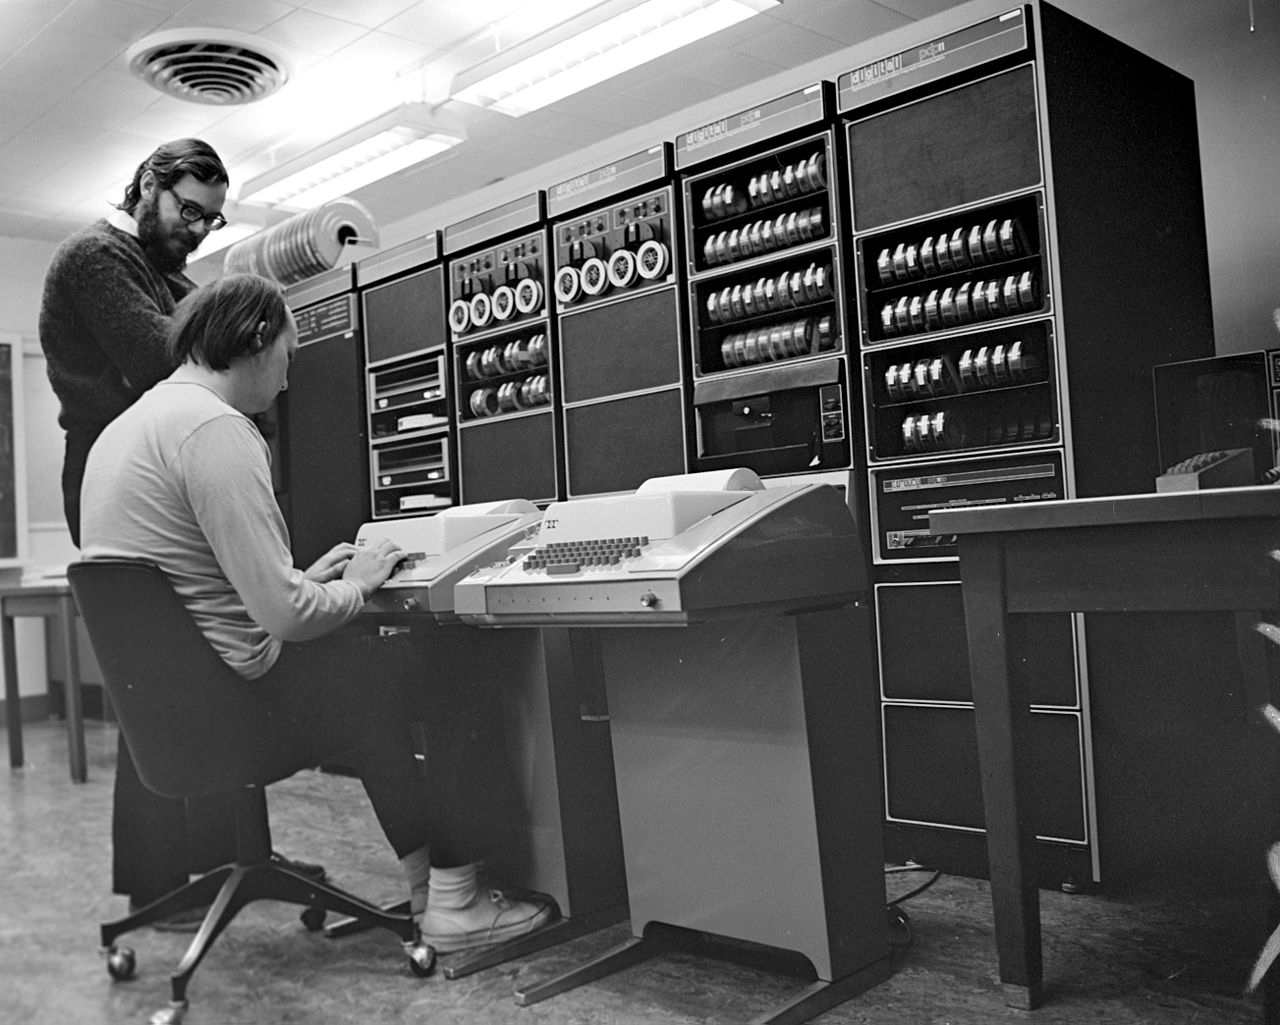
\includegraphics[height=6.4cm]{../pics/Ken_Thompson_(sitting)_and_Dennis_Ritchie_at_PDP-11_(2876612463)}
	\caption{Ken Thompson (sitting) and Dennis Ritchie at PDP-11}
	\end{figure}
}

\frame{
	\frametitle{Short History of Software}
	\framesubtitle{The Awakening of Freedom (\cite{williams:free})}
	\begin{itemize}
		\item Richard Stallman (RMS), \emph{hacker} at the MIT Artificial Intelligence (AI) lab
		\pause
		\item Both the \emph{hacker} and academic cultures are about building, sharing, and improving
		\pause
		\item Suddenly, Xerox shockingly refuses to give the source code so RMS could make it work with the lab's new PDP11
		\pause
		\item RMS sees the printer as a Trojan horse in the AI lab
		\pause
		\item Also the rule of secrecy (NDA) violates \emph{hacker ethics} and the \emph{Golden Rule} (once bound to secrecy, one can't help his/her next of kind)
	\end{itemize}
}

\frame{
	\frametitle{Short History of Software}
	\framesubtitle{The GNU Project and the Free Software Foundation (\cite{rms:GNUproject})}
	\begin{itemize}
		\item in January 1984, RMS quits his job at MIT to write GNU software
		\pause
		\item in 1985, creates the Free Software Foundation (FSF)
		\pause
		\item GNU General Public License
		\pause
		\item \href{https://www.gnu.org/gnu/thegnuproject.html}{Software Freedom Law Center} provides pro-bono legal services to developers of Free, Libre, and Open Source Software.
		\pause
		\item St IGNUcius leads his adepts to the land of Freedoms
	\end{itemize}
}

\frame{
	\frametitle{Short History of Software}
	\framesubtitle{The Four Freedoms (\cite{rms:GNUproject})}
	Quoting from RMS:
	\begin{enumerate}
		\item You have the freedom to run the program as you wish, for any purpose.
		\pause
		\item You have the freedom to modify the program to suit your needs. (To make this freedom effective in practice, you must have access to the source code, since making changes in a program without having the source code is exceedingly difficult.)
		\pause
		\item You have the freedom to redistribute copies, either gratis or for a fee.
		\pause
		\item You have the freedom to distribute modified versions of the program, so that the community can benefit from your improvements.
	\end{enumerate}
}

\frame{
	\frametitle{Short History of Software}
%	\framesubtitle{An introduction to Free/Libre Open Source Software (\href{https://www.youtube.com/watch?v=Tyd0FO0tko8}{Intel, 2014})}
	\framesubtitle{An introduction to Free/Libre Open Source Software (\cite{intel2014:FLOSS})}
	\begin{figure}
	
\includegraphics[height=5cm]{../pics/intel-FLOSS-intro}
	\caption{Credit: Intel Software (2014)\newline{}\url{https://www.youtube.com/watch?v=Tyd0FO0tko8}}
	\end{figure}
}

\frame{
	\frametitle{Short History of Software}
	\framesubtitle{The difference between Free Software and Open Source Software (\cite{osi:history})}
	\begin{itemize}
		\item Open Source appears in 1998, out of a difference of perspective
		\pause
		\item Open Source focuses on the development methodology and its business benefits
		\pause
		\item Free Software makes an ethical statement about user freedom and \emph{rights}
		\pause
		\item Free/Libre Open Source Software (FLOSS) to (over)simplify
	\end{itemize}
}

% --------------------- Software Licensing --------------------------
\subsection{Software Licensing}
\frame{
	\frametitle{Software Licensing}
	\framesubtitle{Copyright \& the need for Licenses}
	\begin{itemize}
		\item IP Laws: Copyright, Patents, Trademark, Trade Secrets
		\pause
		\item Copyright law governs creative works \url{www.cipo.ic.gc.ca/copyrights}
		\pause
		\item Copyright $\neq$ Public Domain
		\pause
		\item Copyright owners (often the authors) are granted exclusive rights for a period of time
		\pause
		\item A license is a legal document that grants some of those rights to others (e.g. software users), seldom under some conditions
		\pause
		\item Software licenses are mostly dealing about copyright
	\end{itemize} 
}

\frame{
	\frametitle{Software Licensing}
	\framesubtitle{Copyright Ownership}
	\begin{itemize}
		\item Individual Contributor
		\pause
		\item Employee working for a company
		\pause
		\item Individuals \& companies might want to assign their copyright (e.g. at the \href{https://www.gnu.org/licenses/why-assign.html}{FSF})
		\pause
		\item Only copyright owners can sue
	\end{itemize}
}

\frame{
	\frametitle{Software Licensing}
	\framesubtitle{Copyleft}
	\begin{itemize}
		\item a twist on ``Copyright''
		\pause
		\item Copyright licenses are often triggered by ``distribution''
		\pause
		\item A spectrum of licenses with diverse conditions \& limitations
			\begin{itemize}
				\item Permissive Licenses (e.g. BSD License)
		\pause
				\item Weak Licenses (e.g. GNU Lesser General Public License)
		\pause
				\item Viral Licenses (e.g. GNU General Public License)
			\end{itemize}
		\pause
		\item Other licenses (e.g. for documentation)
		\pause
		\item Derived works and the chain of title (\cite{rosen2005open})
		\pause
		\item Mixing licenses --the question of license compatibility
	\end{itemize}
}

\frame{
	\frametitle{Software Licensing}
	\framesubtitle{FLOSS License Compatibility (Picture by David A. Wheeler [\href{http://creativecommons.org/licenses/by-sa/3.0}{CC BY-SA 3.0}], via Wikimedia Commons)}
	\begin{figure}
	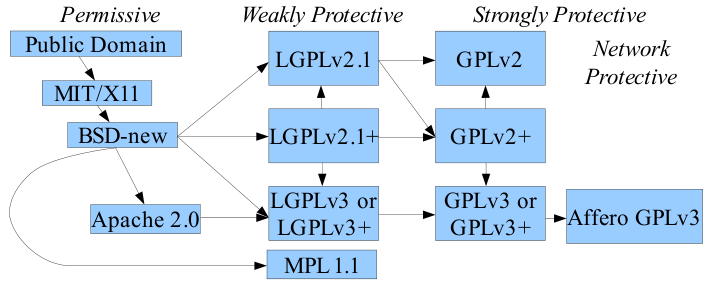
\includegraphics[width=11.5cm]{../pics/Floss-license-slide-image}
	\end{figure}
}

\frame{
	\frametitle{Software Licensing}
	\framesubtitle{Managing Legal Complexity}
	\begin{itemize}
		\item reduce legal risk
		\pause
		\item provide clarity and education
		\pause
		\item best practice: internal company policy (\cite{meeker2008open})
		\pause
		\item understand how that plays out with company strategy
	\end{itemize}
}

\frame{
	\frametitle{Software Licensing}
	\framesubtitle{Example: Odoo}
	\begin{itemize}
		\item AGPL up to Odoo 8.0
		\pause
		\item LGPL from Odoo 9.0 forward --see \href{https://www.odoo.com/blog/odoo-news-5/post/adapting-our-open-source-license-245}{the announcement}
		\pause
		\item A change of business model
		\pause
			\begin{itemize}
				\item AGPL favours system integrators
				\item LGPL favours the individual developers and the growth of an App Store
			\end{itemize}
		\pause
		\item What are the implication of switching to another license? 
	\end{itemize}
}

% --------------------- FLOSS and Business Strategy --------------------------
\subsection{FLOSS and Business Strategy}
\frame{
	\frametitle{FLOSS and Business Strategy}
	\framesubtitle{FLOSS is everywhere}
	\begin{itemize}
		\item 498 out of 500 supercomputers run Linux (see \href{https://www.linux.com/blog/week-open-source-microsoft-expands-open-source-love-498500-supercomputers-run-linux-and-more}{Linux.com, November 2016})
		\pause
		\item Microsoft joined The Linux Foundation as a Platinum Member
		\pause
		\item Close to half the workload on Microsoft Azure run FLOSS
		\pause
		\item FLOSS is in the Space Station, Watches, Cars\ldots
		\pause
		\item Developers seem to take FLOSS for granted
		\pause
		\item The Open Source methodology is proven to be best (e.g. InnerSource at PayPal, HR at WIPRO)
		\pause
		\item GitHub has 14M registered users
		\pause
		\item In 2014, VCs invested \$2.4B into FLOSS-focused companies
	\end{itemize} 
}

\frame{
	\frametitle{FLOSS and Business Strategy}
	\framesubtitle{How to make money with Open Source: some popular business models for providers}
	\begin{figure}
	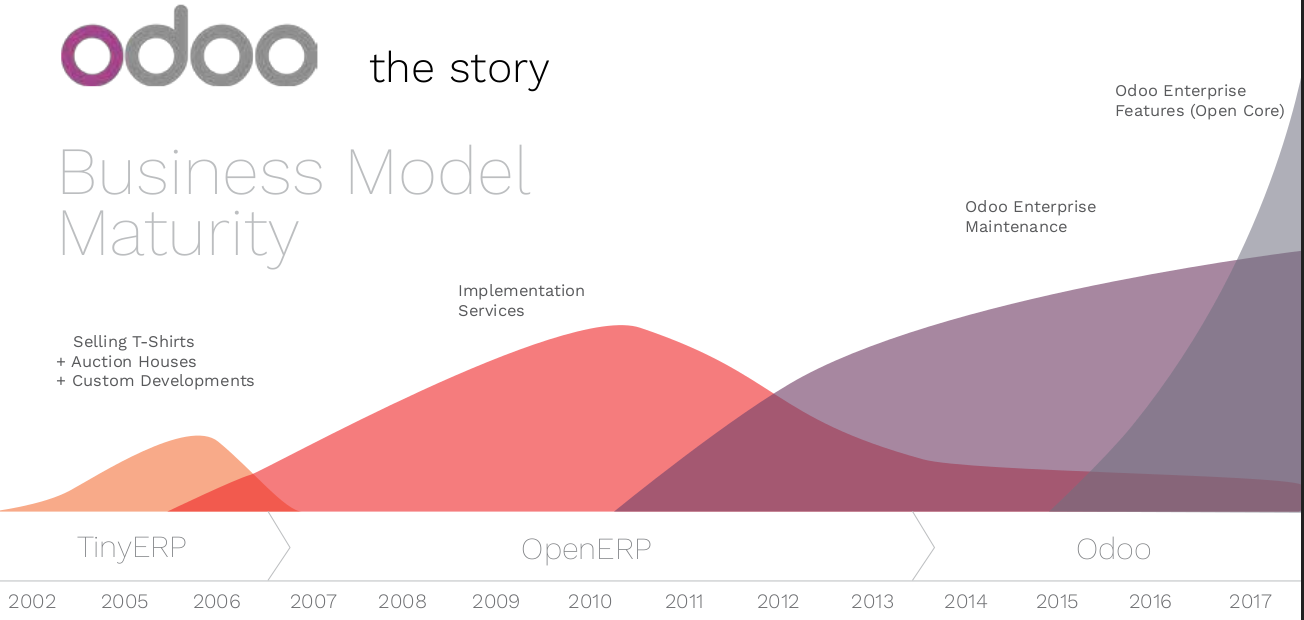
\includegraphics[width=11.5cm]{../pics/odoo-business-model}
	\end{figure}
}

\frame{
	\frametitle{FLOSS and Business Strategy}
	\framesubtitle{How to make money with Open Source: some popular business models for providers}
	\begin{itemize}
		\item Create your start up (e.g. Google, Facebook, Twitter)
		\pause 
		\item System Integrator (e.g. Savoir-faire Linux)
		\pause
		\item Software Publisher (e.g. Odoo SA, Red Hat)
		\pause
		\item Platform play --to generate network externalities (e.g. Google Android, and Chrome/Chromium)
		\pause
		\item Outsourcing and cost-sharing (e.g. CMC and the Bombardier C-Series case study)
		\pause
		\item Setting the pace and imposing standards (e.g. Google Tensor Flow)
		\pause
		\item Software as a Service (e.g. Odoo cloud service)
		\pause
		\item Cutting down cost of R\&D (e.g. Linksys routers, Tom Tom GPS, Bosh)
		\pause
		\item Open Core (e.g. Odoo)
		\pause
		\item Industry Consortiums (e.g. Eclipse, Linux Foundation and its many projects)
	\end{itemize}
}

\frame{
	\frametitle{FLOSS and Business Strategy}
	\framesubtitle{The consumer perspective: how to take advantage of FLOSS}
	\begin{itemize}
		\item Free as in Freedom, and as Free to try (low barrier to adoption) --leading to an innovation culture and technological leadership
		\pause
		\item Extreme customization: fit software to the business, and not the other way around (on the other end proprietary software can be slow to adopt by employees sticking to the old ways)
		\pause
		\item Control cost (in a monopolistic scenario, software vendors can stop investing in R\&D and/or ignore customer complaints)
		\pause
		\item Reduce and eliminate vendor lock-in (asking for APIs, ability to run FLOSS)
		\pause
		\item Security, Privacy, and Control (especially against the ``cloud'' solutions)
		\pause
		\item Sovereign Strategy: maintain and nurture core competencies to secure a competitive advantage
		\pause
		\item Creates and strengthens a local labour market and healthy competition (same as the ability to choose between a car agency and the neighbourhood mechanic)
	\end{itemize}
}

\frame{
	\frametitle{FLOSS and Business Strategy}
	\framesubtitle{Individuals benefit the most from \emph{user rights} and \emph{Freedoms}}
	\begin{itemize}
		\item Privacy vs. Proprietary software ``spying'' (e.g. always-on systems like Amazon Alexa pose a real threat to privacy)
		\pause
		\item Ability to use one's own media vs. DRM and other blocking mechanisms (see \url{https://www.defectivebydesign.org})
		\pause
		\item Software benefits flow down to end-users vs. Tivoization 
		\pause
		\item Equal and fair access to Internet and Computing Resources (e.g. Net Neutrality)
		\pause
		\item Keeping democracies honest and incentivizing civic engagement (e.g. voting machines, Code.org)
	\end{itemize}
}

\frame{
	\frametitle{FLOSS and Business Strategy}
	\framesubtitle{The drawback of FLOSS (\cite{nayafia:roadsandbridges})}
	\begin{itemize}
		\item Key infrastructure projects lack funding (\cite{nayafia:roadsandbridges})
		\pause
		\item Companies could contribute more
		\pause
		\item There are not enough maintainers vs. contributors
		\pause
		\item A lot too many people don't care about licensing (e.g. 85\% of the projects on GitHub don't have a license)
		\pause
		\item Is FLOSS dying from its success (like smartphones are now called phones)? (see \href{https://medium.com/@nayafia/we-re-in-a-brave-new-post-open-source-world-56ef46d152a3\#.7xx10ropr}{Nadia Eghbal})
	\end{itemize}
}

\frame{
	\frametitle{FLOSS and Business Strategy}
	\framesubtitle{Make the world a better place: examples from the \href{http://www.fsf.org/campaigns/priority-projects/}{FSF High Priority List}}
	\begin{itemize}
		\item \href{https://www.fsf.org/campaigns/priority-projects/voicevideochat}{Real-time voice and video chat} -- try \href{https://ring.cx}{Ring beta2} lead by Savoir-faire Linux
		\pause
		\item Free phone operating system (e.g. Replicant removes the pieces that are not free in Android)
		\pause
		\item Better hardware/firmware, drivers, and 3D capabilities
		\pause
		\item Accessibility
		\pause
		\item Security
	\end{itemize}
}

% --------------------- Acquiring an IT Solution --------------------------
\subsection{Acquiring an IT Solution}
\frame{
	\frametitle{Acquiring an IT Solutions}
	\framesubtitle{Consider the pros \&cons of the main options}
	\begin{itemize}
		\item Build
		\pause
		\item Buy (for a time: license)
		\pause
		\item Rent (as a service)
		\pause
		\item Collaborate
		\pause
		\item Other?
	\end{itemize}
}

\frame{
	\frametitle{Acquiring an IT Solutions}
	\framesubtitle{Best choice will depend on the situation}
	\begin{itemize}
		\item Do you even have a choice? Sometimes there is no software out there that fits the bill\ldots
		\pause
		\item How expensive is the alternative out there? (e.g. video processing system developed by Savoir-faire Linux for the TV Industry)
		\pause
		\item Do you have the capabilities (in-house) to build and to maintain a software you need?
		\pause
		\item Are these capabilities a core competency for your business?
		\pause
		\item Is data and intelligence critical to your business?
		\pause
		\item Can you live with a commodity (low-cost) solution that fits somewhat most but not all of your needs?
		\pause
		\item Do you want support locally or are you fine with off-shore support?
	\end{itemize}
}

\frame{
	\frametitle{Acquiring an IT Solutions}
	\framesubtitle{Comparing Apples to Apples}
	\begin{alertblock}{Comparing purchase price of FLOSS vs. Proprietary Solutions}
		FLOSS can be downloaded for free, while proprietary software requires a payment. Their cost structure differs. How do we compare apples to apples?
	\end{alertblock}
}

\frame{
	\frametitle{Acquiring an IT Solutions}
	\framesubtitle{Comparing Apples to Apples: Total Cost of Ownership (TCO)}
	\begin{itemize}
		\item Cost of building or buying
		\pause
		\item Cost of maintainance
		\pause
		\item Cost of replacing (refurbishing, getting the upgrade, migrating data)
		\pause
		\item Cost of tailoring to the business
		\pause
		\item Cost of security
		\pause
		\item Cost of risk (e.g. provider bankrupcy, product phased out, patent case)
		\pause
		\item Cost of the team (HR, facilities)
		\pause
		\item Other costs (see \url{https://www.business-case-analysis.com/total-cost-of-ownership.html})
	\end{itemize}
}

\frame{
	\frametitle{Acquiring an IT Solutions}
	\framesubtitle{Think IT Strategy before planning the procurement process}
	\begin{itemize}
		\item FLOSS can generate 90\% saving \emph{for the right projects} --see \url{http://oss-watch.ac.uk/resources/procurement-infopack}
		\pause
		\item Can big projects be broken down in smaller, manageable projects? (Allow small firms to compete.)
		\pause
		\item Can the intended solution be developed incrementally over time? It is often the best approach for ERP projects, as people need time to learn the system and to adjust their practice.
		\pause
		\item Eliminate unnecessary barriers (leave open door for all types of software, FLOSS or proprietary, and all types of businesses)
		\pause
		\item Have a back-up plan in case the solution goes bust
	\end{itemize}
}

\frame{
	\frametitle{Acquiring an IT Solutions}
	\framesubtitle{Implementing the Solution}
	\begin{itemize}
		\item ERPs deal with business process (i.e. an opportunity for process innovation)
		\pause
		\item Change is hard --use a sound methodology (e.g. \href{http://www.kotterinternational.com/8-steps-process-for-leading-change/}{Kotter's 8-step process})
		\pause
		\item Incremental Innovation: improve a process, then automate it in software, then learn from the new process, then improve it\ldots
		\pause
		\item Example: opening an e-commerce service
	\end{itemize}
}

% ~ ~ ~ References
\frame{
	\frametitle{Creating Value with Software}
	\framesubtitle{References}
	% keyword refers to bib file: references-KEYWORD.bib, and to the Tex file: section-KEYWORD.tex
	\printbibliography[keyword=FLOSS]
}



% Afternoon: 
% (C) Marc Lijour, 2016-2017 
% Licensed under a Creative Commons License BY-SA
% https://creativecommons.org/licenses/by-sa/2.5/ca/
% Presentation for the Small Business Digitization Initiative (SBDI) training program
% see http://www.ictc-ctic.ca/small-business-digitization-initiative/ 
% authored by Marc Lijour, December 2016
% for the session running from January 2017 to September 2017
% 
% ======================================================================================================
%                                      SALARY TRENDS
% ======================================================================================================
\section{Salary Trends}
% --------------------- Definition --------------------------
%\subsection{Why it matters}

\frame{
	\frametitle{Salary discrepancy across regions}
	\begin{figure}	
		\centering
		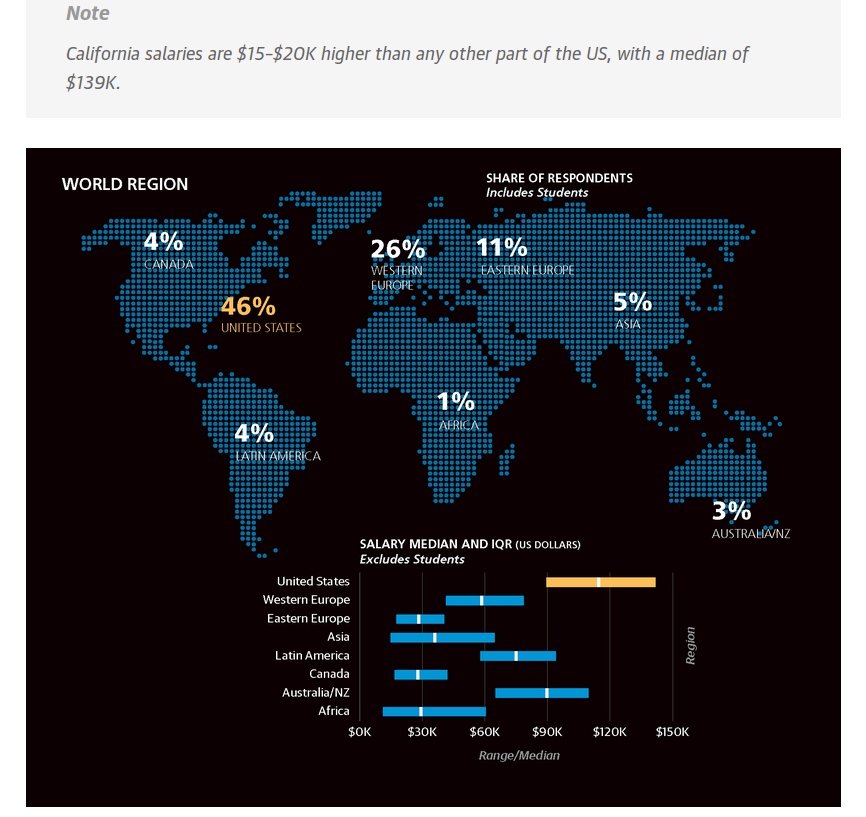
\includegraphics[height=6cm]{../pics/oreilly2017-salary-survey-worldmap}
		\caption{see \href{https://www.oreilly.com/ideas/2017-software-development-salary-survey}{O'Reilly Salary Survey (\cite{oreillysalarysurvey2017})}}
	\end{figure}
}



\frame[allowframebreaks]{
	\frametitle{References}
	%\framesubtitle{References}
	% keyword refers to bib file: references-KEYWORD.bib, and to the Tex file: section-KEYWORD.tex
	\printbibliography[keyword=salary-trends]
}



% (C) Marc Lijour, 2016-2017 
% Licensed under a Creative Commons License BY-SA
% https://creativecommons.org/licenses/by-sa/2.5/ca/
% Presentation for the Small Business Digitization Initiative (SBDI) training program
% see http://www.ictc-ctic.ca/small-business-digitization-initiative/ 
% authored by Marc Lijour, December 2016
% for the session running from January 2017 to September 2017
% 
% ======================================================================================================
%                                   GLOBAL COMPETITION - MACROECONOMIC FORCES
% ======================================================================================================
\section{Global Competition}
% --------------------- Currencies --------------------------
\subsection{Currency Competition}
\frame{
	\frametitle{Global Competition}
	\framesubtitle{Purchasing Power Parity (PPP)}
	\begin{itemize}
		\item Idea that a basket of common goods would have the same pricing value across countries and currencies
		\pause
		\item Assumptions:
			\begin{itemize}
				\item no transaction cost (currency exchange)
		\pause
				\item no trade barriers
			\end{itemize}
		\pause
		\item Useful to think about:
			\begin{itemize}
				\item Arbitrage
		\pause
				\item Undervaluation and overvaluation due to market expectation (e.g. US President Trump \& Mexico)
		\pause
				\item Policies such as currency fluctuation and trade barriers
			\end{itemize}
	\end{itemize}
}

% From the Economist:
% THE Big Mac index was invented by The Economist in 1986 as a lighthearted guide to whether currencies are at their “correct” level. It is based on the theory of purchasing-power parity (PPP), the notion that in the long run exchange rates should move towards the rate that would equalise the prices of an identical basket of goods and services (in this case, a burger) in any two countries. For example, the average price of a Big Mac in America in January 2017 was $5.06; in China it was only $2.83 at market exchange rates. So the ``raw'' Big Mac index says that the yuan was undervalued by 44% at that time. 
\frame{
	\frametitle{Global Competition}
	\framesubtitle{Currency Valuation: \href{http://www.economist.com/content/big-mac-index}{The Big Mac Index (\cite{bigmacindex})}}
	%\framesubtitle{Currency Valuation: \href{http://www.economist.com/content/big-mac-index}{The Big Mac Index}}
	% Discuss: it does not take into account labor cost
	\begin{figure}
	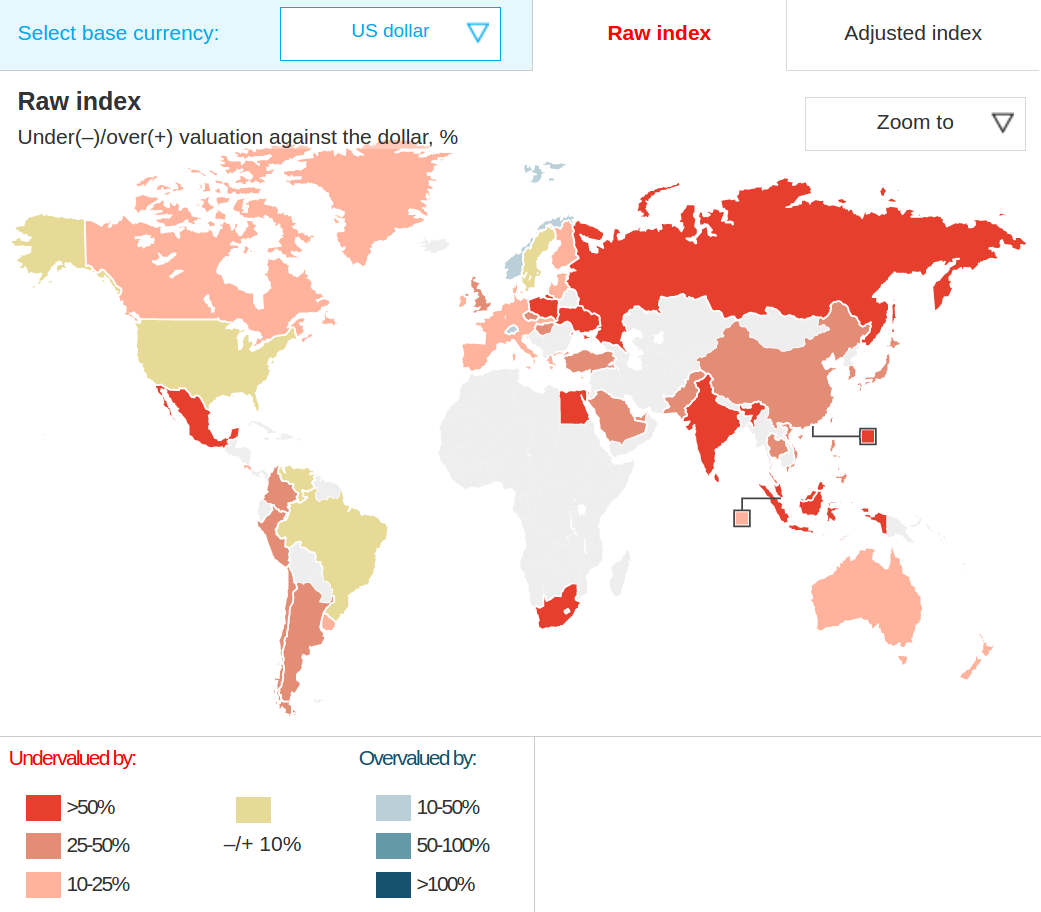
\includegraphics[height=7.5cm]{../pics/big-mac-index}
	\end{figure}
}

% --------------------- Trade Barriers --------------------------
\subsection{Trade Barriers}
\frame{
	\frametitle{Global Competition}
	\framesubtitle{Tariffs}
	\begin{itemize}
		\item Tax on the circulation of goods
		\pause
	\item See Canada's \href{http://www.cbsa-asfc.gc.ca/trade-commerce/tariff-tarif/2017/menu-eng.html}{Customs Tariff (\cite{customstariff2017})}
		\pause
		\item Countries set their own policies, alone or in association (e.g. NAFTA, TPP, CETA)
		\pause
		\item Policies derive from political viewpoints (changing over time), for example
		\pause
			\begin{itemize}
				\item Canada cuts \$48M in tariffs on food ingredients to boost manufacturing, as \href{http://www.cbc.ca/news/politics/food-ingredient-tariff-cuts-1.3942870}{reported on \citejournal{cbc:foodtariff} (January 20, 2017)}
		\pause
	\item US President Trumps threatened German car makers with a 35\% import tariff, as \href{http://business.financialpost.com/news/transportation/trump-threatens-german-carmakers-with-35-u-s-import-tariff}{reported on the \citejournal{fpost:trumpcar} (January 16, 2017)}
			\end{itemize}
		\pause
		\item Impact on the Manufacturing Industry, Global Supply Chain, Foreign Investment, Currencies\ldots
	\end{itemize}
}

\frame{
	\frametitle{Global Competition}
	\framesubtitle{Non-Tariff Barriers}
	\begin{itemize}
		\item Circulation of staff delivering services across borders
		\pause
		\item Licensing (e.g. cryptography)
		\pause
		\item Standards
		\pause
		\item Quotas
		\pause
		\item Labeling and Packaging conditions
		\pause
		\item Intellectual Property Laws (e.g. patents)
		\pause
		\item Protected Designation of Origin (e.g. Champagne, Feta cheese)
	\end{itemize}
}

\subsection{Fiscal Policies}
\frame{
	\frametitle{Global Competition}
	\framesubtitle{Corporate Tax Rates}
	\begin{figure}
	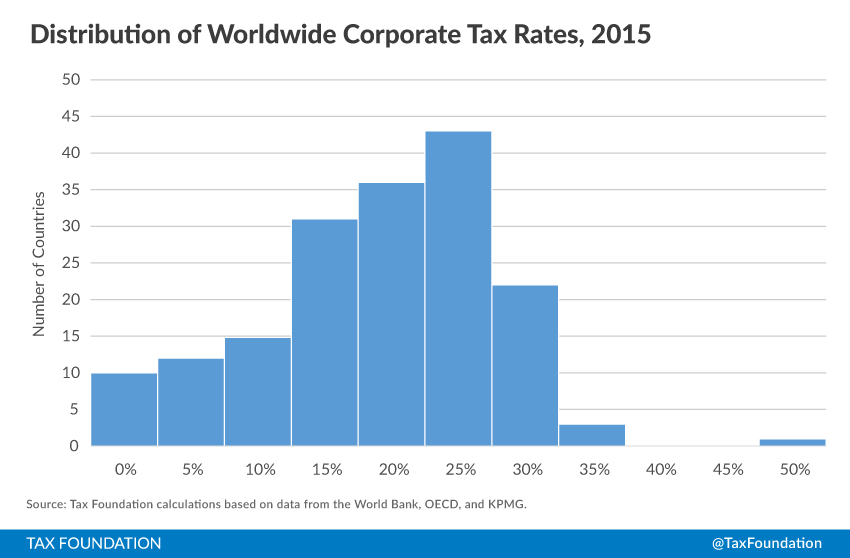
\includegraphics[height=7.5cm]{../pics/taxFoundation2015-worldwide-taxrates}
	\end{figure}
}

\frame{
	\frametitle{Global Competition}
	\framesubtitle{Corporate Income Tax Rates Competition (G7 Top 3 from \href{http://www.investinontario.com/spotlights/canada-ranks-1st-g7-corporate-tax-rate-and-cost-competitiveness}{\cite{kpmg2016}})}
	\begin{figure}
	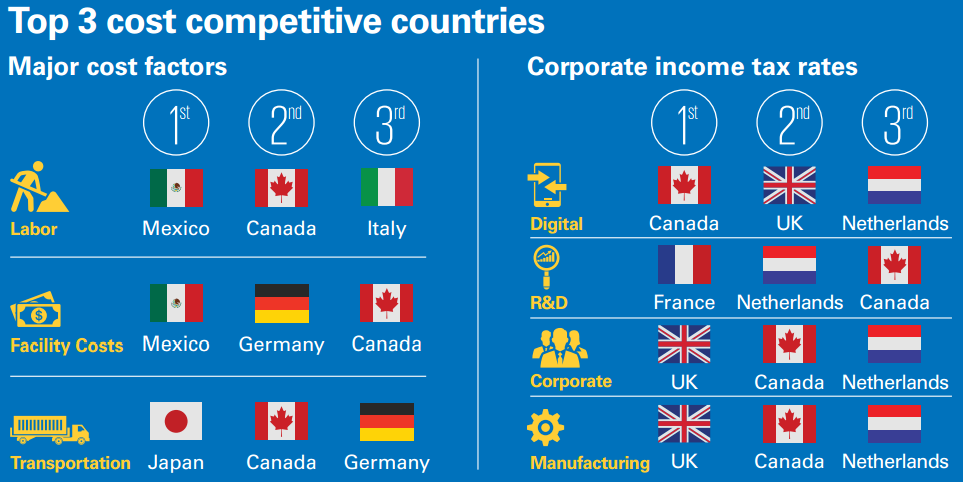
\includegraphics[width=11.5cm]{../pics/KPMG2016-top3-competitive-countries}
	\end{figure}
}

\subsection{Competitiveness Rankings}
\frame{
	\frametitle{Global Competition}
	\framesubtitle{Countries with the lowest business cost (G7 Top 10 from \href{http://www.investinontario.com/spotlights/canada-ranks-1st-g7-corporate-tax-rate-and-cost-competitiveness}{\cite{kpmg2016}})}
	\begin{figure}
	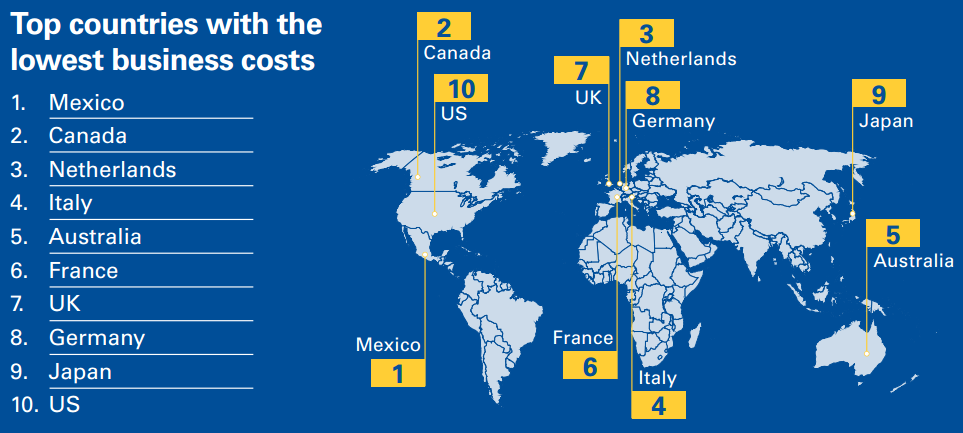
\includegraphics[width=11.5cm]{../pics/KPMG2016-top10-countries-wlow-bizcosts}
	\end{figure}
}

\frame{
	\frametitle{Global Competition}
	\framesubtitle{Business Cost Advantage: Greater Toronto vs USA (York Region, 2016)}
	\begin{figure}
	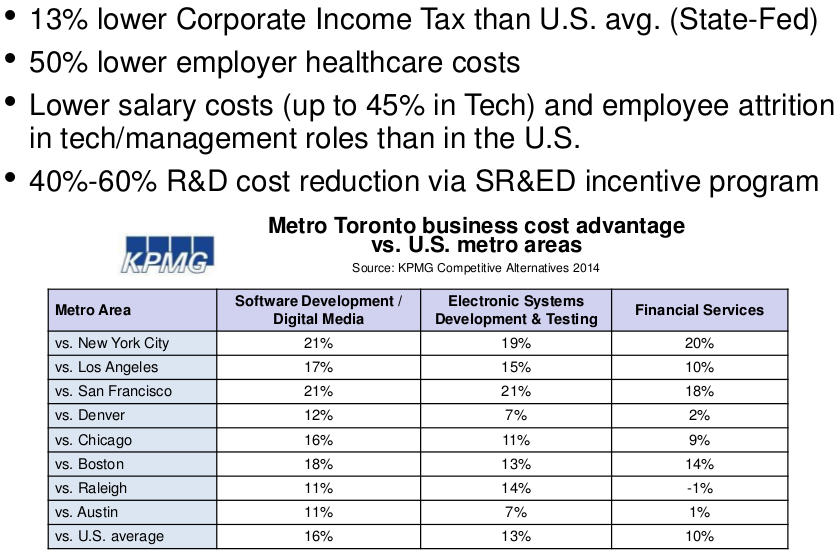
\includegraphics[height=7.5cm]{../pics/York-GTA-cost-advantage-vs-USA}
	\end{figure}
}

\frame{
	\frametitle{Global Competition}
	\framesubtitle{Manufacturing Competitiveness (Global Top 10 from \href{https://www2.deloitte.com/global/en/pages/manufacturing/articles/global-manufacturing-competitiveness-index.html}{\cite{deloitte2016}})}
	\begin{figure}
	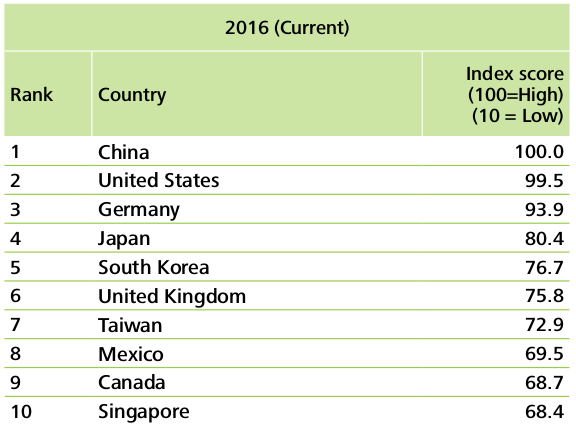
\includegraphics[height=7.5cm]{../pics/deloitte2016-top10-manufacturing-competitiveness}
	\end{figure}
}

\frame{
	\frametitle{Global Competition}
	\framesubtitle{Global Competitiveness Index (Global Top 15 from \href{http://www3.weforum.org/docs/gcr/2015-2016/Global_Competitiveness_Report_2015-2016.pdf}{\cite{wef}})}
	\begin{figure}
	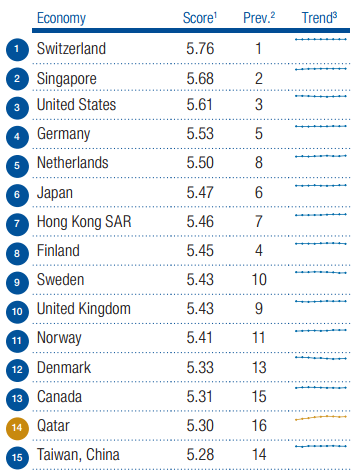
\includegraphics[height=7.5cm]{../pics/wef2016-global-competitiveness-index}
	\end{figure}
}

\frame{
	\frametitle{Global Competition}
	\framesubtitle{VC Money Invested in North American Cities (Thomson Reuters, 2016)} % First nine months of 2016 
	\begin{figure}
	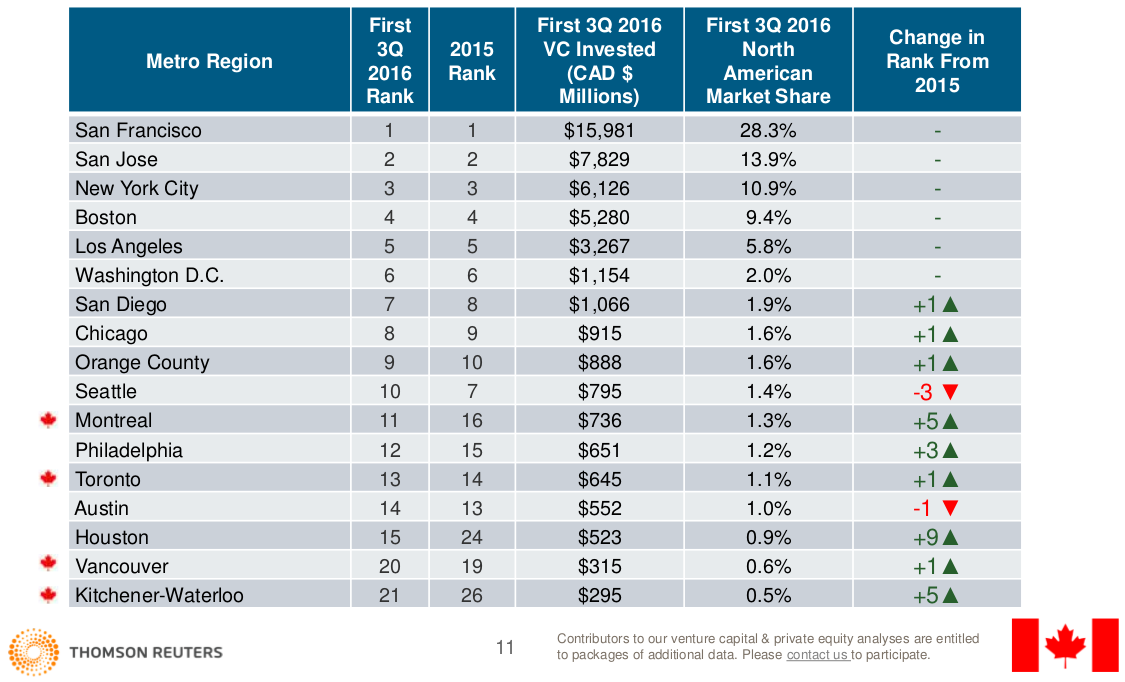
\includegraphics[height=7.4cm]{../pics/thomsonreuters2016-VC-funding-NA}
	\end{figure}
}

\frame{
	\frametitle{Global Competition}
	\framesubtitle{ICT Cluster Density across Canada (York Region, 2016)}
	\begin{figure}
	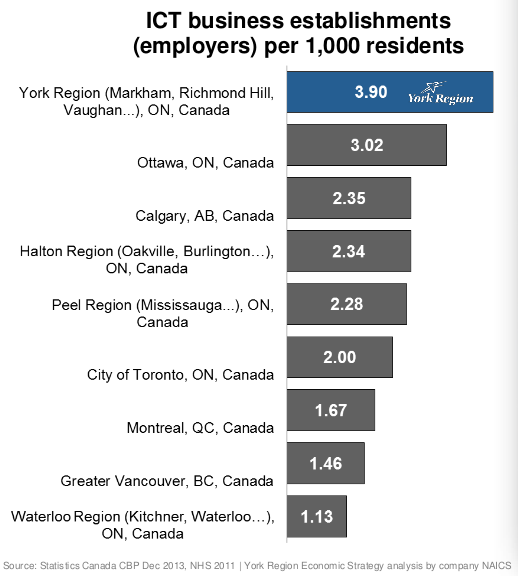
\includegraphics[height=7.5cm]{../pics/York-Canada-ICT-business-density}
	\end{figure}
}

\frame{
	\frametitle{Global Competition}
	\framesubtitle{Size of Ontario ICT Clusters (York Region, 2016)}
	\begin{figure}
	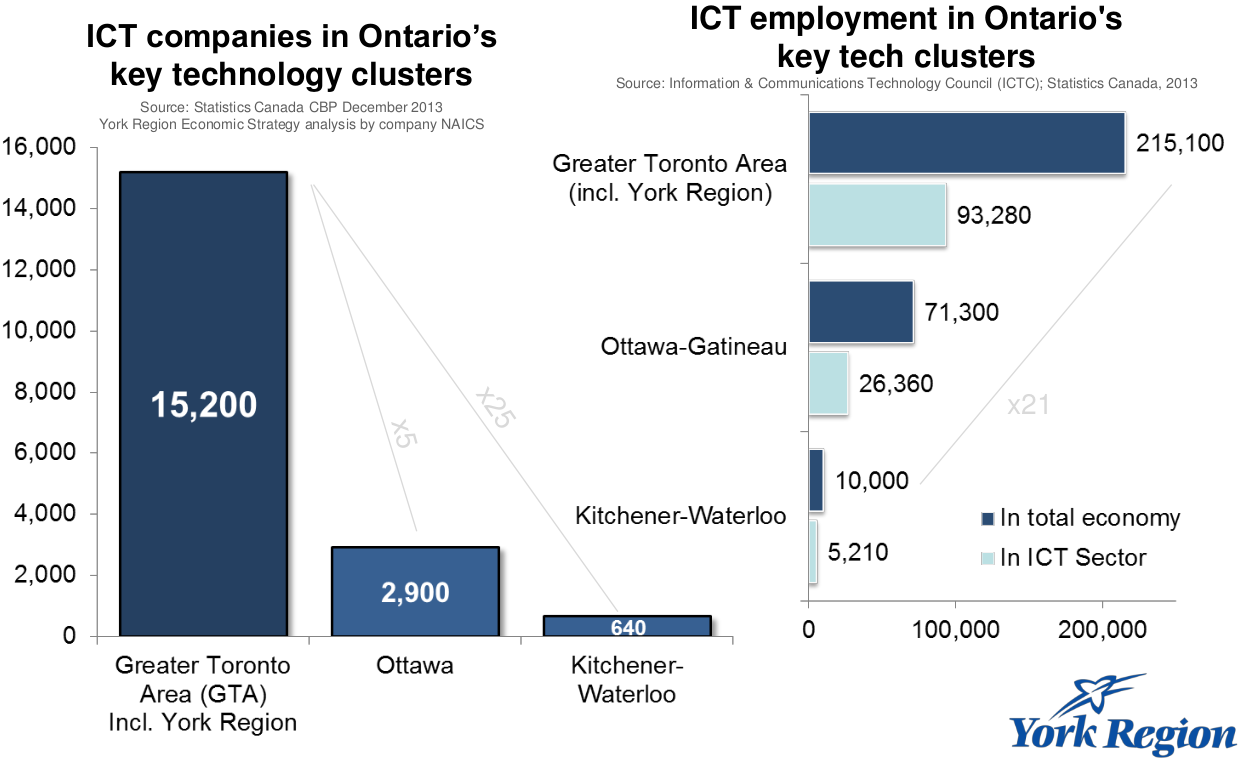
\includegraphics[height=7.4cm]{../pics/York-ICT-cluster-size}
	\end{figure}
}

\frame{
	\frametitle{Global Competition}
	\framesubtitle{Top Canadian Cities by Diversification (\href{https://techtoronto.org/Report2016/}{\cite{techto}})}
	\begin{figure}
	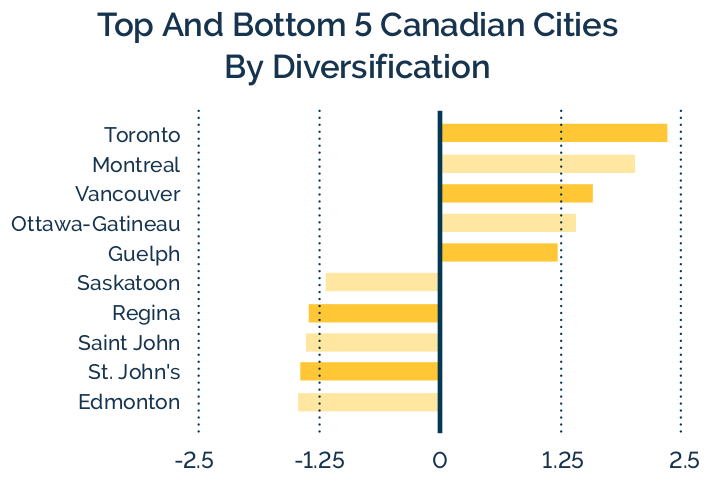
\includegraphics[height=6cm]{../pics/TechTO2016-Top-Canadian-Cities-by-Diversification}
	\end{figure}
}

\frame[allowframebreaks]{
	\frametitle{Global Competition -- References}
	%\framesubtitle{References}
	% keyword refers to bib file: references-KEYWORD.bib, and to the Tex file: section-KEYWORD.tex
	\printbibliography[keyword=global-competition]
}



\end{document}

